\documentclass{amsart}
\usepackage{thomas} % my style file, https://git.io/thomas.sty


\newcommand{\pagenum}{179}
\newcommand{\probnum}{31}

\title{\pagenum.\probnum}
\author{Thomas\ Breydo}

\begin{document}

\maketitle

\begin{problem*}
Use inner products to prove Apollonius's Identity: In a triangle with
sides of length $a,b,$ and $c,$ let $d$ be the length of the line segment
from the midpoint of the side of length $c$ to the opposite vertex. Then
\begin{align*}
    a^2 + b^2 = \frac12 c^2 + 2d^2.
\end{align*}
\end{problem*}
\vspace{0.5in}

Let the triangle be formed by $u,v,u-v\in\R^2$ as shown in the diagram
($z\in\R^2$ is a vector to the ``midpoint'' of $u-v$):
\begin{figure}[h]
    \centering
    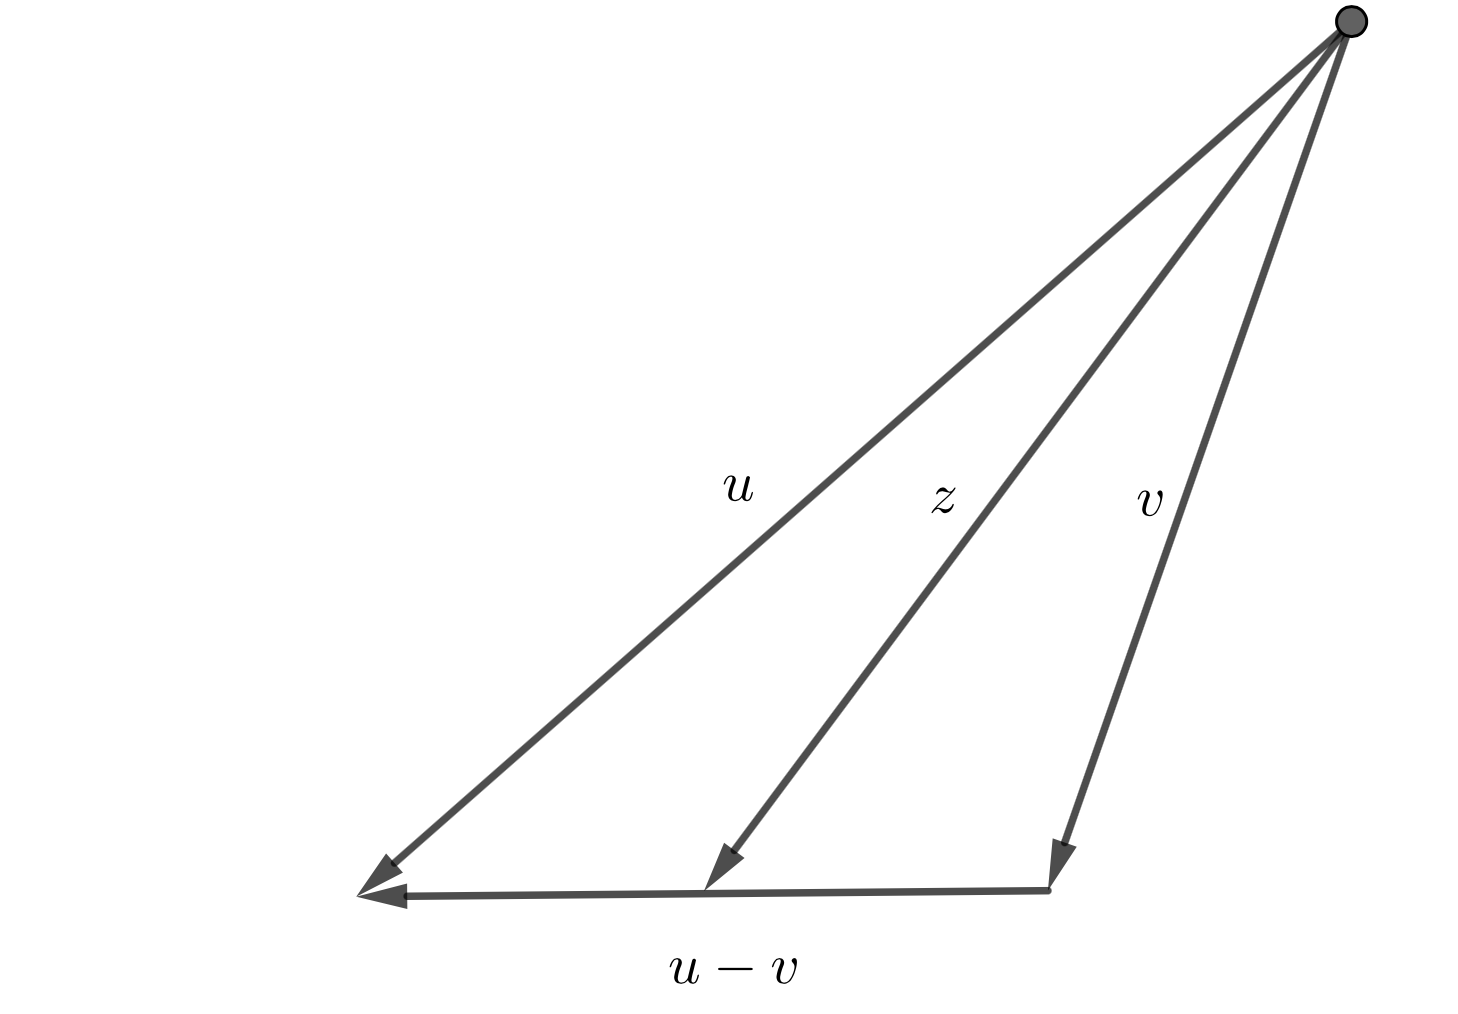
\includegraphics[width=0.85\textwidth]{179_31_triangle.png}
\end{figure}\\
Note that, by construction,
\begin{align*}
    \norm{u} &= a \\
    \norm{v} &= b \\
    \norm{u-v} &= c \\
    \norm{z} &= d.
\end{align*}

\begin{claim*}
    $z=\frac12(u+v).$
\end{claim*}
\begin{proof}
\begin{align*}
    z &= v + \frac{u-v}2 && (by\ definition)\\
      &= \frac{2v+u-v}2 \\
      &= \frac{v+u}2.\qedhere
\end{align*}
\end{proof}

Now that we know what $z$ is, we can prove the identity.
\begin{claim*}
    $a^2+b^2=\frac12c^2+2d^2.$
\end{claim*}
\begin{proof}
Starting tith the right-hand side,
\begin{align*}
    \frac12c^2+2d^2
    &= \frac12\norm{u-v}^2 + 2\norm{z}^2 \\
    &= \frac12\norm{u-v}^2 + 2\norm{\frac12(u+v)}^2 \\
    &= \frac12\norm{u-v}^2 + \frac12\norm{u+v}^2 \\
    &= \frac12\big(
        \iprod{u-v,u-v} + \iprod{u+v,u+v}
       \big) \\
    &= \frac12\big(
        \iprod{u,u} - \cancel{\iprod{u,v}} - \cancel{\iprod{v,u}} 
        + \iprod{v,v} +\iprod{u,u} +\cancel{\iprod{u,v}} +
        \cancel{\iprod{v,u}} + \iprod{v,v}
       \big) \\
    &= \frac12\big( 2\iprod{u,u}+2\iprod{v,v} \big) \\
    &= \iprod{u,u} + \iprod{v,v} \\
    &= \norm{u}^2 + \norm{v}^2 \\
    &= a^2 + b^2.\qedhere
\end{align*}
\end{proof}

\vspace{0.5in}

\begin{note*}
You can view the source code for this solution
\href{https://github.com/thomasbreydo/linalg/blob/main/\pagenum_\probnum_Thomas_Breydo.tex}
{here}.
\end{note*}

\end{document}
